\section{Introduction}
\label{sec:intro}

BGPmon Test Framework  is a collection of software and testing data that tests BGPmon components by running it under various conditions. BGPmon Test Framework has multiple test units that run specific tests and also provide a way to monitor and  analyse results. 

BGPmon Test Framework has following objectives: 
\begin{itemize}
  \item{It should help in automation of BGPmon testing process.}
  \item{It should increase development productivity.}
  \item{It should increase quality of BGPmon components and application.}
  \item{Test units need to include conditions that BGPmon application meet in production environment and conditions that difficult to simulate.}
  \item{It should generate human-readable test reports.}
\end{itemize}

BGPmon Test Framework is designed for  people who interested in testing newly developed or existing components in BGPmon application. BGPmon Test Framework might be interested to people who wants to verify that each particular piece of code that has been written performs the function that it is designed to do. Thus, the audience or users for this document are software developers and quality
managers.
  
%Overall, 
%this  document describes BGPmon Test Framework and its test units. 
%this paper is organized as follows. Section \ref{sec:descr} talks about Test Framework test units. Section \ref{sec:essentials} describes Test Framework essentials: where and how  to start using Test Framework, log options in Test Framework and others.  Section \ref{sec:ipv4peer} describes \emph{IPv4 Peering Test Unit}. It include test unit objectives, unit launch and results reporting.  Section \ref{sec:ipv6peer} introduces \emph{IPv6 Peering Test Unit}. Section \ref{sec:mrt} describes \emph{MRT Module Test Unit} that designed to test MRT module in BGPmon application.  Section \ref{sec:chain} discuss \emph{Chain Modulte Test Unit}. Section \ref{sec:webclient} describes \emph{WebStat Client Test Unit} that tests XML module in BGPmon and provide visual HTML report. 

%Testing framework consist of several test units that are designed for testing BGPmon components and modules.
% like IPv4 and IPv6 peering modules, MRT and Chain modules, WebStat client. 


  
%what is the purpose of the test framework?  
%why we are producing this test framework?

%who is the intended audience?   

%what can they do with it?   

%why would they be using it?


\subsection{BGPmon Test Framework Overview}
\label{sec:current}

%\subsection{Test Units}
\begin{figure}
\centering
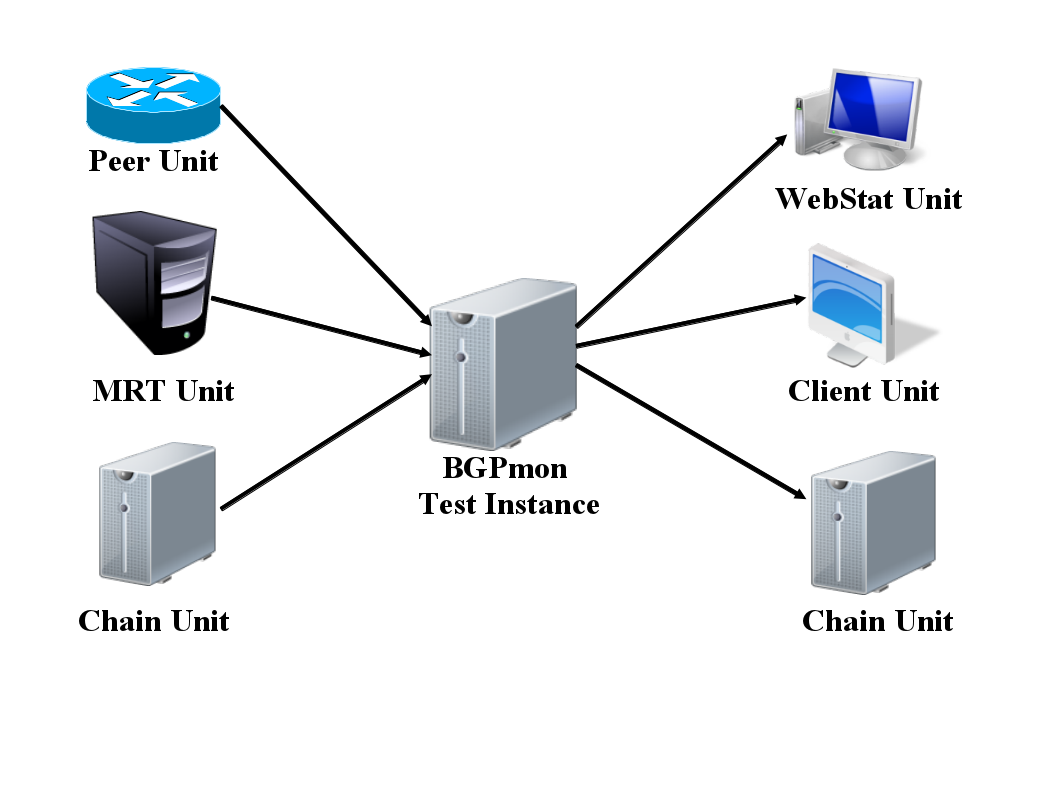
\includegraphics[scale=0.40]{figs/BGPmon-framework-design.png}
\caption{An overview of BGPmon Test Framework architecture.}
\label{designfig}
\end{figure}

Figure \ref{designfig} shows ideal setup of  BGPmon Test Framework that has 7 components.   Test Framework is designed in the way that it tests functionality of  modules in BGPmon application.  BGPmon test instance that shown in the center of the figure  has 3 distinct types of input: \emph{Peer}, \emph{MRT} and \emph{Chain} units.  First, \emph{Peer} unit, sends BGP messages over the BGP peering session.   Second, \emph{MRT} unit, provide BGP messages in MRT format.  \emph{Peer} unit is different from \emph{MRT} unit in the way that \emph{Peer} sends BGP messages that are collected directly from a peer, while \emph{MRT} unit provide data from indirect peer through third party. \emph{Chain} logical unit sends BGP messages in a form of XML messages. \emph{Chain} unit is different from \emph{Peer} and \emph{MRT} because it provides messages from other BGPmons. \emph{Peer}, \emph{MRT} and \emph{Chain} units are shown on the left part of Figure \ref{designfig}.   
BGPmon test instance has three types of output: \emph{WebStat}, \emph{Client} and \emph{Chain} units. All 3 units receive XML messages from BGPmon test instance but use it in different way. \emph{WebStat} unit use XML feed to  generate status report about \emph{Peer}, \emph{MRT} and \emph{Chain} units. \emph{Client} is a setup that used for analysis of XML update messages. \emph{Chain} unit is a separate unit that use XML messages to create a mesh network of BGPmons. \emph{WebStat}, \emph{Client} and \emph{Chain} units are shown on the right part of  Figure \ref{designfig}. 

In order to run over IPv4 and IPv6 communication protocols, design of BGPmon Test Framework need be to be updated by introducing IPv4 and IPv6 units in input and output to BGPmon test instance. Thus, 3 types of input (\emph{Peer}, \emph{MRT} and  \emph{Chain}) and 3 types of output (\emph{WebStat}, \emph{Client} and \emph{Chain})  need to have IPv4 and IPv6 units.  For instance, \emph{Peer} logical unit includes \emph{IPv4 Peer} and \emph{IPv6 Peer} testbeds, \emph{MRT} unit have \emph{IPv4 MRT} and \emph{IPv6 MRT} and so forth.  Thus, BGPmon Test Framework presents complete picture of a testbed that designed to support all distinct types of input and output in BGPmon application.

% Today BGPmon application has support of both IPv4 and IPv6 communication protocols and Test Framework include separate IPv4 and IPv6 logical pieces for each of input sources. Figure \ref{designfig}  shows 6 logical pieces on the left: \emph{IPv4 and IPv6 Peers}, \emph{IPv4 and IPv6 MRTs} and \emph{IPv4 and IPv6 Chains}.   On the right side  of the figure,  Test Framework has elements that receive data from BGPmon application.  It includes installation of \emph{IPv4 and IPv6 WebStat clients}, \emph{IPv4 and IPv6 Generic Clients} and \emph{IPv4 and IPv6 Chains}.    Each logical units  has its own and unique goals to test different components of BGPmon test instance.    

\subsection{Current BGPmon Test Framework Setup}

\begin{figure}
\centering
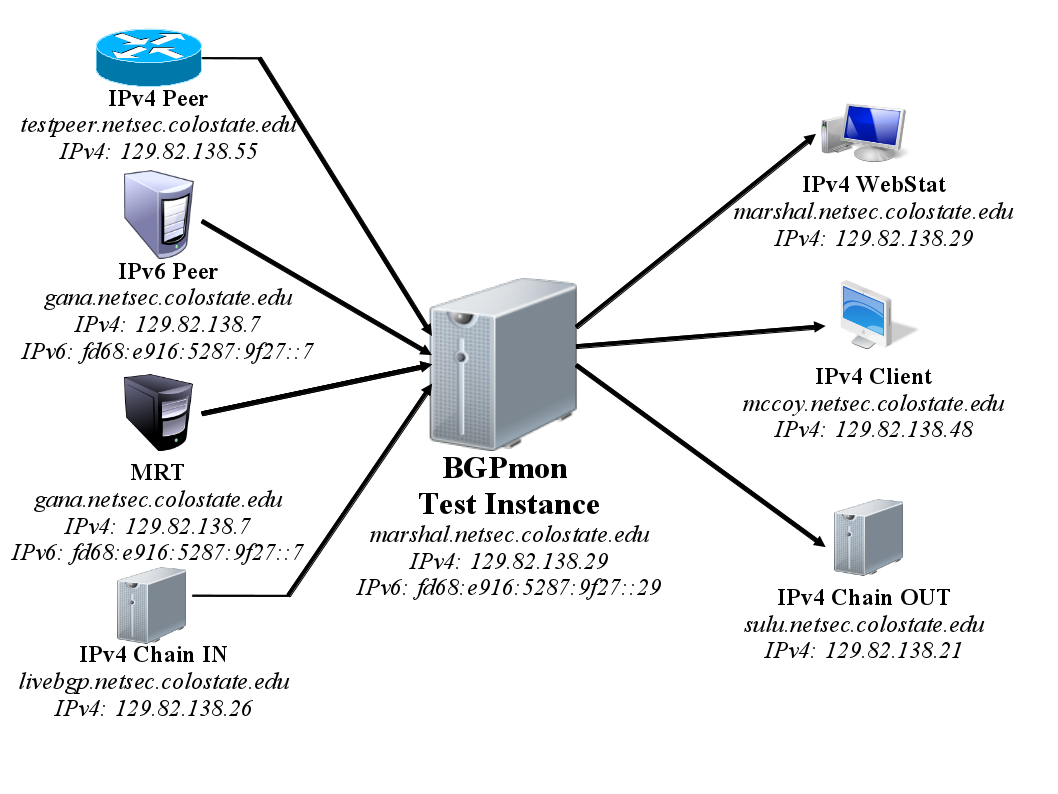
\includegraphics[scale=0.40]{figs/BGPmon-framework-current.png}
\caption{An overview of BGPmon Test Framework architecture.}
\label{currentfig}
\end{figure}

This section describes installation of BGPmon Test Framework and its current status.  Figure \ref{currentfig} shows existing installation and units. BGPmon test instance is installed on \emph{marshal.netsec.colostate.edu} with \emph{129.82.138.29} IPv4 address and \emph{fd68:e916:5287:9f27::101} IPv6 address.        Due to lack of   available equipment and full IPv6 connectivity, existing BGPmon Test Framework setup has limitations and not all logical pieces present in a current installation. 

In Figure \ref{currentfig}, \emph{Peer} unit includes two testbeds: \emph{IPv4 Peer} and \emph{IPv6 Peer} units. \emph{IPv4 Peer} is a setup of Cisco Router and BGPmon instance.  Cisco Router has  \emph{testpeer.netsec.colostate.edu} hostname and \emph{129.82.138.55} IPv4 address.  Despite that this scheme  is designed to test IPv4 peering functionality, it also tests BGPmon  components to receive and process  BGP update messages. Also, \emph{IPv4 Peer} unit is designed to test  BGPmon's efficiency to work with BGP capabilities. \emph{IPv6 Peer} unit is a setup of Quagga Routing Suite software and BGPmon instance. \emph{IPv6 Peer} unit has same goals as \emph{IPv4 Peering}, but it designed to run over IPv6 connectivity.  Quagga software is configured on \emph{gana.netsec.colostate.edu} with two IP addresses: \emph{129.82.138.7} is IPv4 address and \emph{fd68:e916:5287:9f27::101} IPv6 address.  Section \ref{sec:peer} has detailed information about \emph{IPv4 Peer} and \emph{IPv6 Peer} unit goals,  configuration defaults and other. 

\emph{MRT} logical unit includes \emph{IPv4 MRT} testbed that is setup of MRT software and BGPmon test instance.  MRT software is an application that runs on \emph{gana.netsec.colostate.edu} with \emph{129.82.138.7} IP address. MRT application is designed to provide routing data as a third party. In particular, it provides routing data from existing route collectors like Oregon RouteViews project, but it could be used to give routing data from any other MRT source provider.  Section \ref{sec:mrt} has  more details about \emph{IPv4 MRT} unit.

\emph{Chain} logical unit has \emph{IPv4 Chain IN} and \emph{IPv4 Chain OUT} units. First, \emph{IPv4 Chain IN} unit is configuration of BGPmon application that provide stream of table and update messages in a form of XML messages.  \emph{IPv4 Chain IN} runs it on \emph{livebgp.netsec.colostate.edu} and table and update messages are available on ports \emph{50001} and \emph{50002} respectively.  \emph{IPv4 Chain OUT} is setup of BGPmon application that configured to receive XML feed from BGPmon test instance. \emph{IPv4 Chain OUT} is configured on \emph{sulu.netsec.colostate.edu} with \emph{129.82.138.21} IPv4 address.  Thus, \emph{IPv4 Chain IN}, BGPmon test instance and \emph{IPv4 Chain OUT} creates a mesh of BGPmons.  Overall, \emph{IPv4 Chain} that includes both \emph{IPv4 Chain IN} and \emph{IPv4 Chain OUT} units  tests BGPmon's Chain module functionality to create a mesh network of BGPmons, ability of receive and process XML data streams. Section \ref{sec:chain} describes details of this test unit. 

There are 3 types of output that are shown on the right of Figure \ref{currentfig} \emph{WebStat} unit, \emph{Client} unit and \emph{Chain} unit.  

\emph{WebStat} unit include \emph{IPv4 WebStat} testbed that has WebStat software and BGPmon instance.  WebStat software is application that runs on \emph{marshal.netsec.colostate.edu}. WebStat application consist of two components, first, \emph{StatClient} and second, \emph{WebGen}. \emph{StatClient} is application that connects to BGPmon instance and store extracted XML feed in a file system. \emph{WebGen } is unit that generates HTML report that makes summary of configured inputs to BGPmon test instance.  Section \ref{sec:webclient} includes testbed description, test unit goals and others. 

\emph{Client} unit has \emph{IPv4 Client} testbed that is setup of Client software and BGPmon test instance. Client software is application that is configured on \emph{mccoy.netsec.colostate.edu} with \emph{129.82.138.48} IPv4 address. Client software is designed to receive and print XML update messages in a human readable format. Section \ref{sec:client} describes \emph{IPv4 Client} in details. 
 

%Overall, the nature of BGPmon Test Framework Test Units could be divided in two groups: \emph{producers} and \emph{consumers}. \emph{Producers} group include \emph{IPv4 Peering Test Unit}, \emph{IPv6 Peering Test Unit},  \emph{MRT Module Test Unit}  and \emph{Chain Module Test Unit}. \emph{Producers} are the entities that provide data into the system. \emph{Consumers} group include \emph{WebStat Client Test Unit} because this test unit is designed to receive data and analyse it. Thus, the flow of the BGPmon Test Framework could be described in a way that each unit test in \emph{Producers} could be verified with \emph{Consumers} test unit.  For instance, running \emph{MRT Module Test Unit} will generate stream of MRT data that could be easily monitored and analysed using \emph{WebStat Client Test Unit}. Same flow model could be applied to any other test unit in \emph{Producers} group.

\subsection{BGPmon Test Framework Essentials}
\label{sec:essentials}

This sections describes Test Framework Essentials that are important before running any test units. 

Test Framework is configured on \emph{marshal.netsec.colostate.edu}. To get an access to \emph{marshal.netsec.colostate.edu} users of framework need to have access to \emph{bgpmoner} account on \emph{marshal.netsec.colostate.edu}. \emph{bgpmoner} account has all necessary privileges in a system to run or execute Test Framework.  

\subsubsection{BGPmon Launch}

To start using BGPmon Test Framework, BGPmon application has to be launched. To start BGPmon, run following  \emph{init.d} script in a terminal:

\begin{verbatim}
$ sudo /etc/init.d/bgpmon start
\end{verbatim}

This command launches BGPmon application in a background.

To stop using BGPmon Test Framework, stop  BGPmon application:

\begin{verbatim}
$ sudo /etc/init.d/bgpmon stop
\end{verbatim}

\subsubsection{BGPmon Source Code}
Source code of BGPmon application is installed in home directory of \emph{bgpmoner} in following directory:

\begin{verbatim}
/home/bgpmoner/Development/bgpmon-dev
\end{verbatim}

\subsubsection{BGPmon Init.d Script}

Before start using BGPmon application, structure of \emph{init.d} script should be discussed.   \emph{/etc/init.d/bgpmon} script has following definitions:

\begin{verbatim}
BGPMON_EXEC=/usr/local/bin/bgpmon 
CONFIG_FILE=/usr/local/etc/bgpmon_config.txt
PIDFILE=/var/run/bgpmon.pid
ARGS="-d -c $CONFIG_FILE -s -l 7"
\end{verbatim}

\emph{BGPMON\_EXEC} is variable that specifies location of BGPmon executable file. \emph{CONFIG\_FILE} shows location of configuration file that store BGPmon settings.  \emph{PIDFILE} is variable that points to process ID location that is used by \emph{init.d} script. Lastly, \emph{ARGS} is list of command line arguments.   BGPmon application starts with parsing the command line arguments. There are few simple command line arguments that could be specified. In example above, BGPmon uses \emph{-d} to run in daemon world,  \emph{-c \$CONFIG\_FILE} to load default configuration file, \emph{-s} to print log messages to stdlog, \emph{-l 7} defines the log level . In order to debug problems in BGPmon, last two options worth  discussion.

User of the framework may configure BGPmon log functionality to use  \emph{stdout} or \emph{syslog} modes.  First, \emph{stdout mode}, configures BGPmon to run  in an interactive mode that sends all messages to standart output (i.e. terminal).  To enable this option in \emph{init.d}, change \emph{ARGS} line to following:
\begin{verbatim}
ARGS="-d -c $CONFIG_FILE -i -l 7"
\end{verbatim}

Second, \emph{stdlog mode}, configures BGPmon to run in log mode that sends all messages to a file that specified in syslog. \emph{-s} command line argument enables \emph{syslog mode} and \emph{marshal.netsec.colostate.edu} prints log messages to \emph{/var/log/messages} file. To enable \emph{init.d} script use \emph{stdlog mode} use following configuration in \emph{ARGS}:
\begin{verbatim}
ARGS="-d -c $CONFIG_FILE -s -l 7"
\end{verbatim}

BGPmon application  supports different log levels.  \emph{Init.d} script  \emph{/etc/init.d/bgpmon} uses option \emph{-l} with  log value of 7 (\emph{Debug}) and it includes  log values from 0 to 7 (\emph{Emergencies, Alerts, Critical Errors, Errors, Notices, Information, or Debug}). \emph{Debug} provide complete picture of messages that BGPmon application generates. However,  users of framework may configure BGPmon Test Framework log reports to use different levels. This option provides different view of generated logs. For instance, if user  wants to run framework with lower log level like 4 (\emph{Warning}), it need to run \emph{init.d} script with specified log level value. To launch Test Framework with \emph{Warning} log level, change \emph{ARGS} line in \emph{init.d} script to:
\begin{verbatim}
ARGS="-d -c $CONFIG_FILE -s -l 4"
\end{verbatim}

In general, user of framework is free to set any log level value ranging from 0 to 7 by changing \emph{ARGS} value:
\begin{verbatim}
ARGS="-d -c $CONFIG_FILE -s -l logvalue"
\end{verbatim}

%I'm a new developer on BGPmon so I'm looking for you to explain DEBUG to me.       Yes,  I could uncomment this and get something....    not clear why I want to do that?  
%where is this DEBUG?   does setting it one module set it everywhere?
%do want DEBUG in the log or to stdout?
%could I do multiple DEBUG at the same time?
%Jason said in the meeting,  just set DEBUG globally.   is that good or bad?  why?
%am I expected to add my own DEBUG statements as I test?  (answer there is absolutely yes.   does this %document give me enough to understand that?

To truly understand the work flow of components in BGPmon Test Framework, BGPmon application supports modular debugging.  This feature includes critical  messages that are produced by each component during the execution of BGPmon. In order to get the right picture of how components in BGPmon work and communicate between each other, user may enable \emph{DEBUG mode}.  Every source file  in BGPmon home directory has the following macro at the beginning  (after  system libraries linking): 
\begin{verbatim}
//DEFINE DEBUG
\end{verbatim}

Functions in BGPmon components use \emph{controlled text} to print values to stdout. For example:

\begin{verbatim}
#ifdef DEBUG
  debug(__FUNCTION__, "New session with id %d for peer %d", i, peerID);
#endif
\end{verbatim} 

This block is called a \emph{conditional block}. \emph{Debug()} is \emph{controlled text} that will be executed in the output of the preprocessor if and only if \emph{DEBUG} macro is enabled. Most of the functions in BGPmon have at least one conditional block that is wrapped around in  \emph{DEBUG}  macro. 

There are many variants how user can use \emph{DEBUG} macro.  For example, to see  work flow messages from all components, user may recompile BGPmon source code with "-DDEBUG" option. This will enable \emph{DEBUG mode} in each component in BGPmon application.  In this example,  every component would start sending very large amount of log messages to log output and it may create difficulty in understanding and debugging founded problems in BGPmon code.  Instead,  user may uncomment \emph{DEBUG} macro in specific modules. For instance, to enable \emph{DEBUG mode} in \emph{Peering} module in BGPmon application, uncomment \emph{DEBUG} macro :
\begin{verbatim}
//DEFINE DEBUG
\end{verbatim}
to
\begin{verbatim}
DEFINE DEBUG
\end{verbatim}

in each \emph{*.c} source file in \emph{Peering} directory in BGPmon source home directory. To see debug messages, user need to recompile source code and install executable files in a system. In this example,  all \emph{conditional blocks}  that defined in Peering module will be executed.  Also, \emph{DEBUG mode}  functionality could be enabled in any module or groups of modules to debug the problems in BGPmon application. 

However, some users may feel that \emph{DEBUG mode} is not sufficient or  there are too little messages in the output. They can create their own conditional blocks.  Simply,  include conditional block in a function that require additional debugging in source file:
\begin{verbatim}
#ifdef DEBUG
  debug(__FUNCTION__, "Test values are  %d and  %d", value1,  value2);
#endif
\end{verbatim}  

In this example, \emph{debug()} function will print the name of the function (where this block was executed) and two integer values \emph{value1} and \emph{value2} . 

%\subsubsection{BGPmon: Debugging Problems}
%User of Test Framework can debug BGPmon application with set of available tools like \emph{gdb} and %\emph{valgrind}. Those tools can automatically detect memory management problems, threading bugs and %profile your programs in detail.

or what another program was doing at the moment it crashed.
\subsubsection{Test Framework Misconfigurations}

In order to give a complete picture of BGPmon Test Framework Essentials, user need to know about possible misconfigurations in a testbed and further consequences.  Test units in Test Framework might be  configured with any test settings including valid or invalid values. Any misconfigurations  might brake not only test framework setup, but it may affect already working systems.  For example, user may configure to send set of custom MRT update files to \emph{bgpdata.netsec.colostate.edu} hostname  that is not shows on Figure \ref{currentfig}. Results would be tragic, \emph{bgpdata.netsec.colostate.edu} will  provide incorrect data to end clients and it will cause a lot of problems to managers of BGPmon project.  In order to prevent such events, user of framework need to use resources (machines, routers, etc) that are   that are shown on Figure \ref{currentfig} only.   Any usage of other resources is \textbf{strictly forbidden} or it has be discussed with developers and managers of BGPmon project.

%Shell script \emph{/etc/init.d/bgpmon\_startup\_debian.sh} allow user to start and stop BGPmon process. When user run script with ”start” option, it will put BGPmon process in daemon world. Option "stop" with script  terminates BGPmon process using \emph{/var/run/bgpmon.pid} process ID.




%\subsection{Configuration file}
%BGPmon instance load default configuration file \emph{/usr/local/etc/bgpmon\_config.txt}. This file contains internal settings for BGPmon and configuration for BGPmon modules. This file is used every time when user starts or restart BGPmon.  

%\subsection{Logging}
%BGPmon uses \emph{/var/log/messages} file to write all info and debug messages.  

%\subsection{Configuration and Source Code}
%In order to configure BGPmon user has to be logged to \emph{marshal.netsec.colostate.edu}.  BGPmon source code is located in \emph{/home/bgpmoner/Development/bgpmon-dev} directory. To install or reinstall BGPmon, user need to run \emph{./configure \&\& make \&\& sudo make install}.